\documentclass{article}
\usepackage{amsmath}
\usepackage{tikz}
\usetikzlibrary{matrix}

\begin{document}

\[
\sum_{\nu_3,T_3,T_4} 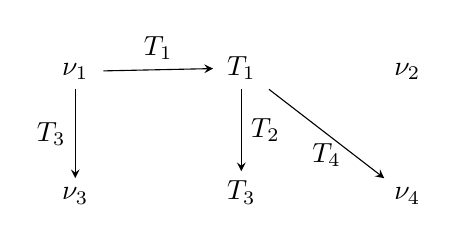
\begin{tikzpicture}[baseline=(current bounding box.center)]
    \matrix (m) [matrix of math nodes,row sep=3em,column sep=4em,minimum width=2em] {
      \nu_1 & T_1 & \nu_2 \\
      \nu_3 & T_3 & \nu_4 \\};
    \path[-stealth]
      (m-1-1) edge node [left] {$T_3$} (m-2-1)
              edge node [above] {$T_1$} (m-1-2)
      (m-1-2) edge node [right] {$T_2$} (m-2-2)
              edge node [below] {$T_4$} (m-2-3);
  \end{tikzpicture}
  \quad
  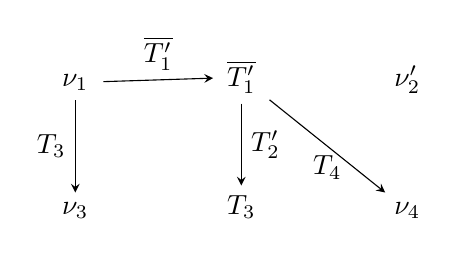
\begin{tikzpicture}[baseline=(current bounding box.center)]
    \matrix (m) [matrix of math nodes,row sep=3em,column sep=4em,minimum width=2em] {
      \nu_1 & \overline{T'_1} & \nu'_2 \\
      \nu_3 & T_3 & \nu_4 \\};
    \path[-stealth]
      (m-1-1) edge node [left] {$T_3$} (m-2-1)
              edge node [above] {$\overline{T'_1}$} (m-1-2)
      (m-1-2) edge node [right] {$T'_2$} (m-2-2)
              edge node [below] {$T_4$} (m-2-3);
  \end{tikzpicture}
  = \delta_{T_1,T'_1} \delta_{T_2,T'_2}
\]

\end{document}